% This is LLNCS.DOC the documentation file of
% the LaTeX2e class from Springer-Verlag
% for Lecture Notes in Computer Science, version 2.4
\documentclass{llncs}
\usepackage{llncsdoc}

\usepackage{graphicx}
%\usepackage{balance}  % for  \balance command ON LAST PAGE  (only there!)
\usepackage{times,amsmath,epsfig,booktabs}
\usepackage[hyphens]{url}
\usepackage{algorithm}
\usepackage{algpseudocode}
%\usepackage{multirow}
\usepackage{listing}
\usepackage{amssymb}
\usepackage{pifont}
\usepackage{verbatim}
%\usepackage{comment}
%\usepackage{subfig}
\usepackage{tikz}
\usepackage{listings}

\usepackage{xcolor,colortbl}

%Hacks to save space
\usepackage{times}
\def\baselinestretch{0.98} 
\usepackage[font={small}]{caption, subfig}
%\usepackage[small,compact]{titlesec}
%\usepackage[small,it]{caption}



\newcommand{\model}{DRAM\_HARD}
\newcommand{\modelExplicit}{DRAM\_SOFT}
\newcommand{\modelPcmRam}{PCM\_RAM}

%\newcommand{\jhcomment}[1]{\noindent {\bf \\JH: #1 \\}}
\newcommand{\jhcomment}[1]{}

\definecolor{c1}{RGB}{239,247,245}
\definecolor{c2}{RGB}{188,189,220}
\definecolor{c3}{RGB}{117,107,177}
\newcolumntype{x}{>{\columncolor{c1}}c}
\newcolumntype{y}{>{\columncolor{c2}}c}
\newcolumntype{z}{>{\columncolor{c3}}c}
%
\begin{document}

\title{
\vspace*{-0.5in}
{\large \bf \hfill
\underline{Second Draft / \today}} \\
\vspace*{0.1in} 
On Improving Write Performance in PCM Databases}
% Three authors sharing the same affiliation.
\author{Vishesh Garg, Abhimanyu Singh, and Jayant R. Haritsa}
%
      \institute {Database Systems Lab, SERC/CSA\\
       Indian Institute of Science, Bangalore, INDIA\\
       \textbf{\email{\{vishesh, abhimanyu, haritsa\}@dsl.serc.iisc.ernet.in}}
       }
          
          
\maketitle
%\markboth{\LaTeXe{} Class for Lecture Notes in Computer
%Science}{\LaTeXe{} Class for Lecture Notes in Computer Science}
%\thispagestyle{empty}
%\begin{flushleft}
%\LARGE\bfseries Instructions for Authors\\
%Coding with \LaTeX\\[2cm]
%\end{flushleft}
%\rule{\textwidth}{1pt}
%\vspace{2pt}
%\begin{flushright}
%\Huge
%\begin{tabular}{@{}l}
%\LaTeXe{} Class\\
%for Lecture Notes\\
%in Computer Science\\[6pt]
%{\Large Version 2.4}
%\end{tabular}
%\end{flushright}
%\rule{\textwidth}{1pt}
%\vfill
%\begin{flushleft}
%\large\itshape
%\begin{tabular}{@{}l}
%{\Large\upshape\bfseries Springer}\\[8pt]
%Berlin\enspace Heidelberg\enspace New\kern0.1em York\\[5pt]
%Barcelona\enspace Budapest\enspace Hong\kern0.2em Kong\\[5pt]
%London\enspace Milan\enspace Paris\enspace\\[5pt]
%Santa\kern0.2em Clara\enspace Singapore\enspace Tokyo
%\end{tabular}
%\end{flushleft}
%

%
\begin{abstract} 

Phase Change Memory (PCM) is a new \emph{non-volatile} memory technology
that is comparable to traditional DRAM with regard to read latency,
and markedly superior with regard to storage density and idle power
consumption. Due to these desirable characteristics, PCM is expected
to play a significant role in the next generation of computing
systems. However, it also has limitations in the form of expensive
writes and limited write endurance. Accordingly, recent research 
has investigated how database engines may be redesigned to
suit DBMS deployments on the new technology.

\begin{comment}
In this paper, we explore the design of PCM-conscious database operators
for main memory organizations comprised of PCM augmented with a small
hardware-controlled DRAM buffer.  Specifically, we present modified
constructions of the ``workhorse'' database operators: \emph{sort},
\emph{hash join} and \emph{group-by}, that substantively improve the
write performance without compromising on execution times. We also
provide \emph{estimators} of the writes incurred by these techniques,
thereby facilitating integration with the database query optimizer.
\end{comment}

In this paper, we explore the design of PCM-conscious database operators
for main memory organizations comprised of PCM augmented with a small
hardware-controlled DRAM buffer. Specifically, we present modified
constructions of the ``workhorse'' database operators: \emph{sort},
\emph{hash join} and \emph{group-by}, which use existing but overlooked ``off-the-shelf'' algorithms for substantively improving the
write performance without compromising on execution times. We also
provide \emph{estimators} of the writes incurred by these techniques,
thereby facilitating integration with the database query optimizer.

The proposed techniques are implemented on a state-of-the-art
architectural simulator, which we extend to model PCM, and their
performance is assessed on a workload of TPC-H benchmark queries. Apart from
the number of writes and query response times, the algorithms are
also evaluated on their wear distributions. Our experimental results
suggest that the PCM-conscious operators collectively reduce the number
of writes by a factor of 2 to 3, while concurrently improving the query
response times by about 20 to 30\%. In essence, our algorithms provide both short-term and
long-term benefits. These outcomes augur well for database engines that
wish to leverage the impending transition to PCM-based computing.

\end{abstract}


\section{Introduction}
\label{sec:intro}
%
Phase Change Memory (PCM) is a recently developed non-volatile memory
technology, constructed from chalcogenide glass material, that stores
data by switching between crystalline (\emph{binary 0}) and amorphous 
(\emph{binary 1}) states. Broadly speaking, it is expected to provide an attractive
combination of the best features of conventional disks (persistence,
capacity) and of DRAM (access speed). For instance, it is
about 2 to 4 times denser than DRAM, while providing a DRAM-comparable
read latency.  On the other hand, it consumes much less energy
than magnetic hard disks while providing substantively smaller write latency. Due to this suite of  desirable features, PCM technology is
expected to play a prominent role in the next generation of computing
systems, either augmenting or replacing current components in the memory
hierarchy~\cite{qureshi,zhou,lee}.

A limitation of PCM, however, is that there is a significant difference
between the read and write behaviours in terms of energy, latency and
bandwidth. A PCM write, for example, consumes 6 times more energy than
a read. Moreover, PCM has limited write endurance since a memory cell
becomes unusable after the number of writes to the cell exceed a threshold
determined by the underlying glass material. Consequently, several database
researchers have, in recent times, focused their attention on devising
new implementations of the core database operators that are adapted to
the idiosyncrasies of the PCM environment (e.g.~\cite{chen,viglas}). 

%\newpage
\subsection*{Architectural Model}
The prior database work has primarily focused on computing
architectures wherein either (a) PCM completely replaces the
DRAM memory~\cite{chen}; or (b) PCM and DRAM co-exist side-by-side
and are independently controlled by the software~\cite{viglas}. We
hereafter refer to these options as {\bf \modelPcmRam{}} and
{\bf \modelExplicit{}}, respectively.

However, a third option that is gaining favor in the architecture
community is where the PCM is augmented with a small hardware-managed
DRAM buffer~\cite{qureshi}. In this model, which we refer to as
{\bf \model{}}, the address space of the application maps to PCM and the
DRAM buffer can simply be visualized as yet another level of the existing
cache hierarchy.  For ease of comparison, these various configurations
are pictorially shown in Figure~\ref{fig:pcm_models}.

\begin{figure}[htbp]
	\includegraphics[height=50mm]{PCM_Models.png}\centering
	\caption{PCM-based Architectural Options}
	\label{fig:pcm_models}
\end{figure}

There are several practical advantages of the \model{} configuration:
First, the write latency drawback of \modelPcmRam{} can be largely
concealed by the intermediate DRAM buffer~\cite{qureshi}. Second,
existing applications can be used \textit{as is} but still manage to take
advantage of both the DRAM and the PCM. This is in stark contrast to the
\modelExplicit{} model which requires incorporating additional machinery,
either in the program or in the OS, to distinguish between data mapped
to DRAM and to PCM -- for example, by having separate address space
mappings for the different memories.

\subsection*{Our Work}
We make the following contributions in this paper:
\begin{itemize}
\item Propose PCM-conscious off-the-shelf implementations of the ``workhorse'' database operators:
\textit{sort}, \textit{hash join} and \textit{group-by}, that are tuned to the \model{} model, that reduce
\emph{both} query writes and response times.

\item Incorporate major extensions in Multi2sim \cite{multi2sim},
a state-of-the-art architectural simulator, to support the modelling of PCM.  



\item Evaluate the proposed implementation on \emph{complete} TPC-H benchmark queries.This is a noteworthy point since earlier studies of PCM databases had only
considered operator performance in isolation.  But, it is possible that
optimizing a specific operator may be detrimental to other downstream
operators that follow it in the query execution plan. For instance,
the proposal in \cite{chen} to keep nodes unsorted in B$^+$ indexes,
while saving on writes, can be detrimental to the running times of
subsequent operators, e.g. join filters, that leverage index ordering. The metric of \emph{wear  distribution} is also included in our evaluation.


\item Provide simple but effective mathematical \emph{estimators} for the
number of writes incurred by the new operators and then incorporate them in the query optimizer's
cost model.

\end{itemize}

We observe that the alternate implementations collectively offer
substantive benefits with regard to PCM writes -- the number is typically
brought down \emph{by a factor of two to three}.  Concurrently, the query
response times are also brought down by about \emph{20 to 30 percent}. Overall, these outcomes augur well for the impending migration of database
engines to PCM-based computing platforms.

 
 
 
\begin{comment}
 Our 

The experimental results suggest that, as compared to the original
PCM-oblivious operators, 
As a sample case in point, for TPC-H Query 19, savings of 64\% in PCM
writes are achieved with a concomitant 32\% reduction in CPU cycles.

A unique feature of our analysis is that we also . This is because
a skewed distribution adversely impacts the endurance of cells with high
write rates, raising the frequency at which wear-leveling mechanisms
have to be put into play by the system. We observe that our algorithms don't introduce any new skew while achieving the reduction in writes and cycles.

Finally, 

In a nutshell, the new PCM-conscious operators proposed in this paper
provide both \emph{short-term and long-term performance benefits}.

\end{comment}

\section{Problem Framework}
\label{assumptions}
In this section, we overview the problem framework, the assumptions made
in our analysis, and the notations used in the sequel.

As mentioned in the Introduction, we model the \model{} memory
organization (Figure~\ref{fig:pcm_models} (c)). The DRAM buffer is of
size $D$ and is organized in a \emph{K-way set-associative} manner, like the higher level cache memories.
A \textit{data-comparison write (DCW)} scheme \cite{write} is used for
the writing of PCM memory blocks during eviction from DRAM -- in this
scheme, the memory controller compares the existing PCM block to the newly
evicted DRAM block, and selectively writes back only the modified words.
Further, \textit{N-Chance}~\cite{nchance} is used as the DRAM eviction
policy -- here, the first clean way in the $N$ least recently used ways
(assuming $N$ is less than $K$, the DRAM cache associativity) in a set
is chosen as the eviction victim. Only when all the $N$ ways are dirty,
the LRU entry is evicted. We choose this scheme due to its preference
for evicting non-dirty entries over dirty candidates, thereby saving
on writes.

As described above, the simulator implements a realistic DRAM
buffer. However, in our write analyses and estimators, we assume for
tractability that there are no conflict misses in the DRAM. Thus, for
any operations dealing with data whose size is within the DRAM capacity,
our analysis assumes no evictions and consequently no writes.

With regard to the operators, we use $R$ to denote the input relation
for the \textit{sort} and \textit{group-by} unary operators.  Whereas,
for the binary \textit{hash join} operator, $R$ is used to denote the
smaller relation, on which the hash table is constructed, while $S$
denotes the probing relation. 

We assume that all the input relations are completely PCM-resident.
Further, for simplicity of presentation, we assume that the sort,
hash-join and group-by expressions are on single relational attributes --
the extension to multiple attributes is straightforward.

A summary of the main notation used in the analysis of the following
sections is provided in Table~\ref{tab:notations}.

\begin{table}[!h]
\centering
\caption{Notations Used in Operator Analysis}
\label{tab:notations}
\begin{small}
\begin{tabular}{p{2cm}p{9cm}}
\toprule  
\textbf{Term} & \textbf{Description}\\ 
\midrule
\textbf{$D$} & DRAM size\\
\textbf{$K$} & DRAM Associativity\\
\textbf{$P$} & Pointer size\\
\textbf{$N_R, N_S$} & Row cardinality of relations R and S, respectively\\
\textbf{$L_R, L_S$} & Tuple size of relations R and S, respectively\\
\textbf{$B$} & Number of buckets in hash table\\
\textbf{$size_{entry}$} & Size of each hash table entry\\
\textbf{$J,G$} & Output tuple cardinalities of join and group-by operators, respectively\\
\textbf{$size_{j},size_{g}$} & Output tuple sizes of join and group-by operators, respectively\\
\bottomrule
\end{tabular}
\end{small}
\end{table}


\section{The Sort Operator}
\label{sort}

The quicksort algorithm is the commonly used sorting algorithm in database systems. In the
single pivot quicksort algorithm with $n$ elements, the average number
of swaps is of the order of $0.3nln(n)$~\cite{swaps}. If the initial array is much larger than the DRAM size, it would
entail evictions from the DRAM during the swapping process of
partitioning. These evictions might lead to PCM writes if the evicted
DRAM lines are \textit{dirty}, which is likely since elements are being
swapped. If the resulting partition sizes continue to be larger than
DRAM, partitioning them in turn will again cause DRAM evictions and
consequent writes. Clearly, this trend of writes will continue in the
recursion tree until the partition sizes become small enough to fit within
DRAM. Thereafter, there would be no further evictions during swapping
and the remaining sorting process would finish within the DRAM.

From the above discussion, it is clear that it would be desirable for a sorting algorithm to be in-place, converge fast to partition sizes within DRAM size with less amount of swaps. We pick an alternate algorithm - flashsort \cite{flashsort} - which has these properties. Specifically, flashsort can potentially form DRAM sized partitions in a \emph{single} partitioning step with at most $N_R$ swaps. The sorting is done in-place with a time complexity of $O(N_Rlog_2N_R)$ with constant extra space\footnote{The time complexity can be brought down to $O(N_R)$ with $O(N_R)$ extra space}. The flashsort algorithm proceeds in three phrases: \emph{Classification Phase}, \emph{Permutation Phase} and \emph{Short-range Ordering Phase}. The classification phase divides the input data into $p$ partitions where $p$ is given as input. Given an element with value $v$, $Partition(v) = 1 + \lfloor \frac{(p-1)(v- v_{min})}{v_{max}-v_{min}} \rfloor$; $v_{min}$ and $v_{max}$ being the smallest and the largest values in the array, respectively. It then counts the number of elements in each such partition to get the boundary information. The permutation phase moves the elements to their respective partitions. The individual partitions are then finally sorted in the Short-range Ordering Phase to get the overall sorted array.

We choose the number of partitions $p$ to be $\lceil c \times \frac{N_R L_R}{D} \rceil$, where $c \geq 1$ is a design
parameter, to cater to the possibility that some partitions might turn out to be larger than the DRAM size if the data is not uniformly distributed. In our experience, setting $c = 2$ worked well in practice.

%\input{read_phase_algo}

For partitions that turn
out to be within the DRAM size, the Short-range Ordering phase is completed using
quicksort. On the other hand, if some larger-sized
partitions still remain, we recursively apply the flashsort
algorithm to sort them until all the resulting partitions fit within DRAM and finish sorting with lesser evictions.

\textbf{PCM write analysis}: Though the partition boundary counters
are continuously updated during the Classification phase, they are expected to
incur very few PCM writes. This is because since all those updates are
in quick succession, the counters are unlikely to be evicted from DRAM
\emph{during} the update process. During the
Permutation phase, there will be no more than $N_R L_R$ writes since each tuple is written
at most once while placing it within its partition boundaries. If each
partition is within the DRAM size, the Short-range Ordering phase (for each partition)
will finish within DRAM and there will be another $N_R L_R$ writes upon
eventual eviction of sorted partitions to PCM. 

Thus, for the case of uniform data distribution, the writes incurred by this algorithm is estimated by
\begin{equation}
\label{eq:sort}
  W_{sort} = 2N_RL_R
\end{equation}

\section{The Hash Join Operator}
\label{hj}
Hash join is perhaps the most commonly used of all join algorithms in
database systems. Here, a hash table is built on the smaller relation,
and tuples from the larger relation are used to probe for matching values
in the join column. Since we assume the table is completely PCM-resident, the join here \emph{does not} require any initial partitioning stage. Instead, we directly proceed to the join phase. Thus, during the progress of hash join,
writes will be incurred during the building of the hash table, and also
during the writing of the join results.

Each entry in the hash table consists of a pointer to the corresponding
build tuple and the hash value for the join column. Due to the
absence of prior knowledge about the distribution of join column values
for the build relation, the hash table is expanded dynamically according
to the input. Typically, for each insertion in a bucket, a new space is
allocated and is connected to existing entries using a pointer. Thus,
such an approach incurs an additional pointer write each time a new
entry is inserted.

Our first modification is to use a well-known technique of allocating space to hash buckets in units of \textit{pages} \cite{paging}. A page is of a fixed size and contains a set of contiguous
entries, the maximum count of entries being fixed depending on the size
of the page and the size of the entry. When a page overflows a new page
is allocated and linked to the overflowing page via a pointer.  Thus,
unlike the conventional hash table wherein each \emph{pair} of entries
are connected using pointers, the interconnecting pointer here is only
at page granularity. Note that although open-addressing is another alternative for avoiding pointers, probing for a join attribute value would have to search through the entire table each time, since the inner table might contain \emph{multiple} tuples with the same join attribute value.

A control bitmap is used to indicate whether each entry in a page is vacant
or occupied, a necessary information during both insertion and search in the
hash table. Each time a bucket runs out of space, a new page is allocated
to the bucket. Though such an approach  may lead to space wastage when
some of the pages are not fully occupied, we save on the numerous pointer
writes that are otherwise incurred when space is allocated on a per-entry basis.

Secondly, we can reduce the writes incurred due to storing of the hash values in
the hash table by restricting the length to just a single byte. In this
manner, we trade-off precision for fewer writes. If the hash function
distributes the values in each bucket in a perfectly uniform manner, it
would be able to distinguish between $2^8 = 256$ join column values in a
bucket. This would be sufficient if the number of distinct values mapping
to each bucket turn out to be less than this value. Otherwise, we would
have to incur the penalty (in terms of latency) of reading the actual join
column values from PCM due to the possibility of false positives.

\textbf{PCM write analysis}: We ignore the writes incurred while initializing each hash table bucket since they are negligible in comparison to inserting the actual entries. Assuming there are $E_{page}$ entries per page, there would now be one pointer per $E_{page}$ entries. Additionally, for each insertion, a bit write would be incurred due to the bitmap update. The join tuples would also incur writes which is given by $J \times size_j$. Thus, the total writes for hash join would be
$$W_{hj} = N_R \times (size_{entry} +  \frac{P}{E_{page}} + \frac{1}{8} ) + J \times size_{j}$$
Since in practice both  $\frac{P}{E_{page}}$ and $\frac{1}{8}$ are small as compared to $size_{entry}$, 
\vspace{-0.05in}
\begin{equation}\label{eq:hj}
 W_{hj} \approx N_R \times size_{entry} + J \times size_{j} 
\end{equation} 


\section{The Group-By Operator}%
\label{gby}
We now turn our attention to the group-by operator which typically
forms the basis for aggregate function computations in SQL queries.
Common methods for implementing group-by include \textit{sorting} and
\textit{hashing} -- the specific choice of method depends both on the
constraints associated with the operator expression itself as well as
on the operators following later in the plan tree.

In the following subsections, we begin by considering the hash-based
group-by operator and present our modifications of this technique for
the PCM environment. Subsequently, we move on to a similar discussion
for sort-based group-by implementation. In both these algorithms, the writes due to \emph{output} tuples, is $G \times size_g$.

\subsection{Hash Based Grouping}

A hash table entry for group-by, as compared to the corresponding
entry in hash join, has an additional field containing the aggregate
value. For each new tuple in the input array, a bucket index is
obtained after hashing the value of the column present in the group-by
expression. Subsequently, a search is made in the bucket indicated by
the index. If a tuple matching the group-by column value is found, the
aggregate field value is updated; else, a new entry is created in the
bucket. Thus, unlike hash join, where each build tuple had its individual
entry, here the grouped tuples share a common entry with an aggregate
field that is constantly updated over the course of the algorithm.

Since the hash table construction for group-by is identical to that
of the hash-join operator, the PCM-related modifications described
in Section~\ref{hj} can be applied here as well. That is, we employ
a page-based hash table organization, and a reduced hash value size,
to reduce the writes to PCM.

\textbf{PCM write analysis}: From the above discussion, it is easy to see
that the total writes incurred for the PCM-conscious hash based group-by is given by
\begin{equation}
\label{eq:gb_ht}
\begin{split}
W_{gb\_ht} = G \times size_{entry} + 
N_R \times size_{agg\_field} + G \times size_g
\end{split}
\end{equation}

\subsection{Sort Based Grouping}

Sorting may be used for group-by when a fully ordered operator such
as \textit{order by} or \textit{merge join} appears downstream in the plan
tree. Another use case is for queries with a \textit{distinct} clause
in the aggregate expression, in order to identify the duplicates that have
to be discarded from the aggregate.  

Sorting based group-by differs in a key aspect from sorting itself
in that that the sorted tuples do not have to be written out. Instead, it
is the aggregated tuples that are finally passed on to the next operator
in the plan tree. Hence, we can modify the flashsort algorithm of
Section~\ref{sort} to use \emph{pointers} in both the
\textit{Permutation} and \textit{Short-range ordering} phases, subsequently leveraging these
pointers to perform aggregation on the sorted tuples. 

\textbf{PCM write analysis}: The full tuple writes of $2 N_R L_R$
which were incurred in the flashsort scheme, are
now replaced by $2N_R \times P$ since pointers are used during
both the partitioning and sorting phases. Thus, the total writes for this
algorithm for uniformly distributed data would be:
\begin{equation}
\label{eq:gb_sort}
W_{gb\_sort} = 2N_R \times P + G \times size_g
\end{equation}

\label{sec:exp}

\section{Simulation Testbed}
This section details our experimental settings in terms of the hardware
parameters, the database and query workload, and the performance metrics
on which we evaluated the algorithms.



\subsection{Architectural Platform}
Since PCM memory is as yet not commercially available, we
have taken recourse to a simulated hardware environment to
evaluate the impact of the PCM-conscious operators.  For this
purpose, we chose Multi2sim~\cite{multi2sim}, an open source
application-only\footnote{Simulates only the application layer without
the OS stack.} simulator that can model a multithreaded, multicore,
superscalar x86 CPU and an AMD Evergreen GPU. It has support for both
functional simulation and cycle-accurate detailed architecture simulation.

We evaluated the algorithms on Multi2sim in cycle-accurate simulation
mode. Since it does not have native support for PCM, we made a major
extension to its existing memory module to model PCM memory. Specifically,
the following enhancements were incorporated in the simulator to conduct
our experimental evaluation:

\textbf{Hybrid Main Memory}: 
The memory organization was extended such that the new configuration
consists of PCM with a hardware controlled DRAM buffer. The DRAM buffer
acts as another level of cache in the memory hierarchy, specifically
between the L2 cache and the PCM.

\textbf{New DRAM Replacement Policy}: 
The DRAM is simulated as a set-associative write-back memory with
\textit{N-Chance} as the eviction policy. As mentioned in \cite{nchance},
$N$ was set to $\frac{K}{2}$, where $K$ is the cache associativity,
since this setting was found to provide good performance on multiple
metrics -- writes, energy and latency.

\textbf{Tracking DRAM-PCM Data}:
Like most other architectural simulators, Multi2sim does not explicitly
track the data residing at the different levels of the memory
hierarchy. It instead maintains only a single buffer that indicates
the latest data, as visible to the simulated program, for each memory
location. We therefore had to add separate data tracking functionality
for the DRAM and PCM resident data.

\textbf{Data Comparison Write Scheme}: 
The write-back mechanism of data from DRAM to PCM was modelled on the
DCW~\cite{write} scheme. Thus, for each evicted DRAM block, a comparison
to the original PCM resident data block was made, and writes were
restricted to only those words where the data bits differed. In our
experiments, we measured writes at \textit{word} (4B) granularity.

\textbf{Asymmetric Read-Write Latencies}:  
The timing simulation was modified to account for the higher write
latency of PCM as compared to a read.

\textbf{Wear Distribution}: 
Apart from the raw number of writes, a critical related metric for PCM
algorithms is their wear distribution. We therefore instrumented the
Multi2sim code to track block level wear distribution information. To
achieve this, separate counters were created that tracked writes to each
PCM \textit{line} (256B) during the query processing activity.

\textbf{Intermediate Statistics}: 
Multi2sim does not have support to track intermediate statistics during
a program run. We therefore provided additional inter-process communication capabilities in the
tool so that the simulated program could ask the simulator to dump
statistics for each intermediate operator during the execution of a query.


\begin{center}
\begin{table}[t]
\begin{small}
\caption{Experimental Setup}
\label{table:setup}
\begin{tabular}{p{2.5cm}p{10cm}}
\toprule
Simulator & Multi2sim-4.2 with added support for PCM\\ \hline

L1D cache (private) & 32KB, 64B line, 4-way set-associative, 4 cycle latency, write-back, LRU\\ \hline
L1I cache (private) & 32KB, 64B line, 4-way set-associative, 4 cycle latency, write-back, LRU\\ \hline   
L2 cache (private) & 256KB, 64B line, 4-way set-associative, 11 cycle latency, write-back, LRU\\ \hline

DRAM buffer (private) & 4MB, 256B line, 8-way set-associative, 200 cycle latency, write-back, N-Chance(N = 4)\\ \hline

Main Memory & 2 GB PCM, 4KB page, 1024 cycle read latency (per 256B line), 64 cycle write latency (per 4B modified word)\\ \bottomrule
\end{tabular}
\end{small}
\end{table}
\end{center}

\vspace{-0.4in}
The specific configurations used in the memory hierarchy (L1 Data,
L1 Instruction, L2, DRAM Buffer, PCM) evaluated in our experiments are
enumerated in Table~\ref{table:setup}.  These values are scaled down
versions, wrt number of lines, of the hardware simulation parameters used
in \cite{wear} -- the reason for the scaling down is to ensure that the
simulator running times are not impractically long. However, we have been
careful to ensure that the \emph{ratios} between the sizes of adjacent
levels in the hierarchy are maintained as per the original configurations
in \cite{wear}.  

\begin{comment}
Further, note that the read-to-write latency ratio is
1:4, significantly lower than the 1:20 of Table ~\ref{tab:tab_pcm_char}
in the Introduction. We wish to point out that this makes our results
\emph{conservative} -- if the ratio is made 1:20, the performance
improvements of the new algorithms  are even more substantial.
\end{comment}



%\vspace*{0.05in}

\subsection{Database and Queries}
%We used TPC-H (version 2.16.0) 1GB PCM-resident database for our experiments.
For the data, we used the default 1GB database generated by the TPC-H
benchmark.  This size is certainly small compared to the database sizes
typically encountered in modern applications -- however, we again chose
this reduced value to ensure viable simulation running times.

For simulating our suite of database operators -- \textit{sort},
\textit{hash join} and \textit{group by} -- we created a separate library
consisting of the native PostgreSQL implementation of these operators. To
this library, we added the PCM-conscious versions described in the
previous sections.

While we experimented with several of the TPC-H queries, results for
three queries: Query 13 (Q13), Query 16 (Q16) and Query 19 (Q19), that
cover a diverse spectrum of the experimental space, are presented here.
For each of the queries, we first identified the query execution plan
recommended by the PostgreSQL query optimizer with the native operators,
and then forcibly used the same execution plan for their PCM-conscious
replacements as well. This was done in order to maintain fairness in the
comparison of the PCM-oblivious and PCM-conscious algorithms, though it
is possible that a better plan is available -- we return to this issue 
later in Section~\ref{discussion}. 
%The three SQL queries are enumerated in Figure~\ref{fig:queries}, and their associated execution plans are shown in Figure~\ref{fig:plan_trees}.
The execution plans associated with the three queries are shown in Figure~\ref{fig:plan_trees}. 
 


\begin{figure*}[t]
\centering
\subfloat[Q13]{
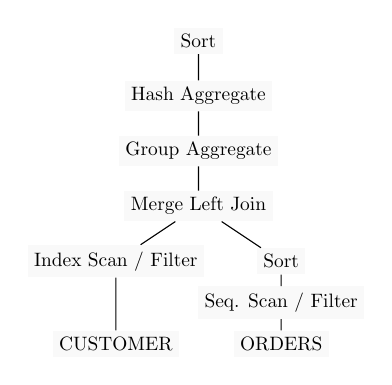
\begin{tikzpicture}[scale=.7, transform shape]

\tikzstyle{every node} = [rectangle, fill=gray!5]

\node (d) at (0,3) {Index Scan / Filter};
\node (c) at (0,1.5) {CUSTOMER};

\node (s) at (3,3) {Sort};
\node (p) at (3,2.25) {Seq. Scan / Filter};
\node (a) at (3,1.5) {ORDERS};

\node (e) at (1.5,4) {Merge Left Join};
\node (f) at (1.5,5)  {Group Aggregate};
\node (g) at (1.5,6)  {Hash Aggregate};
\node (h) at (1.5,7)  {Sort};


\draw[-] (c) -- (d);
\draw[-] (a) -- (p);
\draw[-] (d) -- (e);
\draw[-] (p) -- (s);
\draw[-] (s) -- (e);
\draw[-] (e) -- (f);

\draw[-] (f) -- (g);
\draw[-] (g) -- (h);

\end{tikzpicture}
}
\subfloat[Q16]{
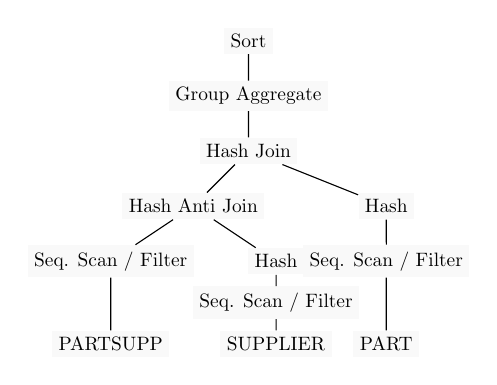
\begin{tikzpicture}[scale=.7, transform shape]

\tikzstyle{every node} = [rectangle, fill=gray!5]

\node (d) at (0,3) {Seq. Scan / Filter};
\node (c) at (0,1.5) {PARTSUPP};

\node (s) at (3,3) {Hash};
\node (p) at (3,2.25) {Seq. Scan / Filter};
\node (a) at (3,1.5) {SUPPLIER};

\node (e) at (1.5,4) {Hash Anti Join};

\node (n) at (5, 4) {Hash};
\node (b) at (5,3) {Seq. Scan / Filter};
\node (x) at (5,1.5) {PART};

\node (f) at (2.5,5)  {Hash Join};
\node (g) at (2.5,6)  {Group Aggregate};
\node (h) at (2.5,7)  {Sort};


\draw[-] (c) -- (d);
\draw[-] (a) -- (p);
\draw[-] (d) -- (e);
\draw[-] (p) -- (s);
\draw[-] (s) -- (e);
\draw[-] (e) -- (f);

\draw[-] (x) -- (b);
\draw[-] (b) -- (n);
\draw[-] (n) -- (f);

\draw[-] (f) -- (g);
\draw[-] (g) -- (h);

\end{tikzpicture}

}
\subfloat[Q19]{


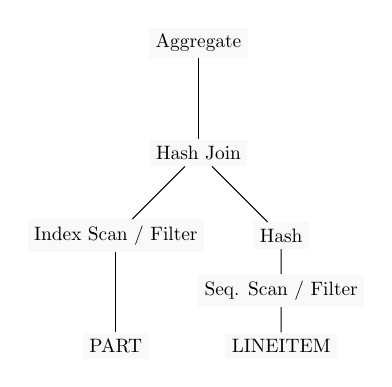
\begin{tikzpicture}[scale=.7, transform shape]

\tikzstyle{every node} = [rectangle, fill=gray!5]

\node (d) at (0,3.5) {Index Scan / Filter};
\node (c) at (0,1.5) {PART};

\node (s) at (3,3.5) {Hash};
\node (p) at (3,2.5) {Seq. Scan / Filter};
\node (a) at (3,1.5) {LINEITEM};

\node (e) at (1.5,5) {Hash Join};
\node (f) at (1.5,7)  {Aggregate};


\draw[-] (c) -- (d);
\draw[-] (a) -- (p);
\draw[-] (d) -- (e);
\draw[-] (p) -- (s);
\draw[-] (s) -- (e);
\draw[-] (e) -- (f);
\end{tikzpicture}
}

\caption{ Query execution plan trees}

\label{fig:plan_trees}

\end{figure*}




\subsection{Performance Metrics}
We measured the following performance metrics for each of the queries:
\begin{description}


\item [PCM Writes:] The total number of word (4B) updates that are applied to the PCM memory during
the query execution.
\item [CPU Cycles:] The total number of CPU cycles required to execute the query.
\item [Wear Distribution:] The frequency of writes measured on a per-256B-block basis.

\end{description}

\section{Experimental Results}
\label{sec:results}
Based on the above framework, we conducted a wide variety of experiments
and present a representative set of results in this section.

We begin by profiling the PCM Writes and CPU Cycles behavior of
the native and PCM-conscious executions for Q13, Q16 and Q19 --
these results are shown in Figure ~\ref{fig:overall_results}.  In each of these figures, we provide both the total and
the break-ups on a per operator basis.

\begin{figure*}[t]

\centering

\subfloat[Impact of sort on overall performance - Q13]{
  \includegraphics[height=29mm]{overall_q13.png}
  
}
\hspace{0mm}
\subfloat[Impact of group-by on overall performance - Q16]{
  \includegraphics[height=29mm]{overall_q16.png}
}
\hspace{0mm}
\subfloat[Impact of hash join on overall performance - Q19]{
  \includegraphics[height=29mm]{overall_q19.png}
}
\caption{Overall performance of queries}
\label{fig:overall_results}
\end{figure*}


Focusing our attention first on Q13 in
Figure~\ref{fig:overall_results}(a), we find that the bulk of the
overall Writes and Cycles are consumed by the Sort operator. Comparing
the performance of the Native (blue bar) and PCM-conscious (green bar)
implementations, we observe a very significant savings (53\%) on Writes,
and an appreciable decrease (20\%) on Cycles.

Turning our attention to Q16 in Figure~\ref{fig:overall_results}(b),
we find that here it is the group-by operator that primarily influences
the overall Writes performance, whereas the hash-join determines the
Cycles behavior. Again, there are substantial savings in both Writes
(40\%) and  Cycles (30\%) delivered by the PCM-conscious approach.

Finally, moving on to Q19 in Figure~\ref{fig:overall_results}(c),
where hash-join is essentially the only operator, we find that the
savings are around $64\%$ with regard to Writes and $32\%$ in Cycles.

\subsection{Operator-wise Analysis}
We now analyse the savings due to each operator independently, and show
their correspondence to the analysis in Sections~\ref{sort}--\ref{gby} .

\paragraph{Sort}
For Q13, as already mentioned, we observed savings of $53\%$ in writes and
$20\%$ in cycles.  In the case of Q16, the data at the sorting stage was
found to be much less than the DRAM size. Hence, both the native and
PCM-conscious executions used the standard sort routine, and as a result,
the cycles and writes for both implementations match exactly.

\paragraph{Hash Join}
Each entry in the hash table consisted of a pointer to the build tuple
and a hash value field. New memory allocation to each bucket was done
in units of pages, with each page holding up to 64 entries. A search for
the matching join column began with the first tuple in the corresponding
bucket and went on till the last tuple in that bucket, simultaneously
writing out the join tuples for successful matches.  For Q16, we
observed a $34\%$ improvement in Writes and $12\%$ in Cycles due to the
PCM-conscious hash join, as shown in Figure~\ref{fig:overall_results}(b).
These improvements were even higher with Q19  -- 65\% Writes and 32\%
Cycles in Figure~\ref{fig:overall_results}(c) -- the source of the
enhancement was the 3 bytes of writes saved due to single-byte hash
values, in addition to the page-based aggregation of hash table entries.


\paragraph{Group-By}
In Q16, the aggregate operator in the group-by has an associated
\textit{distinct} clause.  Thus, our group-by algorithm utilized
hash-based in-place partitioning followed by sorting to carry out the
aggregation. Both the partitioning and sorting were carried out through
pointers, thereby reducing the writes significantly. Consequently,
we obtain savings of $74\%$ in Writes and $20\%$ in Cycles, as shown
in Figure~\ref{fig:overall_results}(b).  When we consider Q13, however,
the hash table consisted of very few entries. The less number of entries
led to the overhead of the page metadata construction overshadowing the
savings obtained in other aspects. Specifically, only marginal improvements
of about 4\% and 1\% were obtained for Writes and Cycles, as shown in
Figure~\ref{fig:overall_results}(a).

\begin{figure*}[t]
\centering

\subfloat[Q13]{
  \includegraphics[width=4cm]{wear_q13.png}
}
\subfloat[Q16]{
  \includegraphics[width=4cm]{wear_q16.png}
}
\subfloat[Q19]{
  \includegraphics[width=4cm]{wear_q19.png}
}
\caption{Queries wear distribution }
\label{fig:wear_dist}
\end{figure*}



\subsection{Lifetime Analysis}
\begin{comment}
In \cite{qureshi}, the ideal lifetime $Y$ of a PCM device with size $S$
GB, $B$ write traffic, and cell endurance $W_{max}$, is given by:

$Y(years) = \frac{W_{max} \times S}{B} \times 2^{-25}$\\
\end{comment}

The above experiments have shown that PCM-conscious operators
can certainly provide substantive improvements in both Writes and
Cycles. However, the question still remains as to whether these
improvements have been purchased at the expense of \emph{longevity} of
the memory. That is, are the writes skewed towards particular memory
locations?  To answer this, we show in Figure~\ref{fig:wear_dist}, the
maximum number of writes  across all memory blocks (as mentioned earlier,
we track writes at the block level (256 bytes) in our modified simulator),
for the three TPC-H queries. The x-axis displays the block numbers in
decreasing order of writes.

We observe here that the maximum writes is considerably more for the
native systems as compared to the PCM-conscious processing. This
conclusively demonstrates that the improvement is with regard to
\emph{both} average case and worst case behavior.

\subsection{Validating Write Estimators}
\label{validation}

We now move on to validating the estimators
(presented in Section~\ref{sort} through \ref{gby})  for the number of
writes incurred by the various database operators.

\subsubsection{Sort}
The size of the $orders$ table is approximately $214 \times 10^6$ bytes. 
The PCM-conscious version used multi-pivot sort algorithm and
incurred writes of $110.6 \times 10^6$ words $= 441.8 \times 10^6 $
bytes. Replacing the values for $N_R L_R$ in Equation \ref{eq:sort},
we get the writes as 
\begin{small}
$$W_{sort}(bytes) \approx 2 \times 214 \times
10^6  = 428 \times 10^6 $$ 
\end{small}
Thus the estimates are close to the
observed writes.



\subsubsection{Hash Join}
For the hash join in Q19, the values of $N_R$, $size_{entry}$, $J$,
$size_{j}$ are $2 \times 10^5$, $5$, $120$ and $8$, respectively. 
For the PCM-conscious version, the estimated writes are given by Equation \ref{eq:hj},
and substituting  the  parameter values, the writes are given by:  
\begin{small}
$$W_{hj}(bytes) = 2 \times 10^5 \times 5 + 120 \times 8 \approx 10^6$$
\end{small}
which is close to the actual writes of $0.32 \times 10^6$ words $=
1.28 \times 10^6$ bytes.

\begin{table}[t]                                                                                       
\centering                                                                                              
\caption{Validation of Write Estimators}
  \label{tab:estimator_validation}                                                                                
  %\centering                                                                                             
  \begin{small}                                                                                           
  \begin{tabular}{p{3cm}p{3cm}p{3cm}p{2.5cm}}
  \toprule                                                                                                
  
  \textbf{Operator} & \textbf{Estimated Writes} (e) & \textbf{Observed Writes} (o) & \textbf{Error Factor} $\frac{e-o}{o}$\\
  \midrule                                                                                                
  
    \textbf{Sort} &  $428 \times 10^6$ & $441.8 \times 10^6$ & -0.03\\ 
  \textbf{Hash Join} &  $1 \times 10^6$ & $1.28 \times 10^6$ & -0.22\\ 
  \textbf{Group-By} &  $1.83 \times 10^6$ &$1.44 \times 10^6$ & 0.27\\ 
  
  \bottomrule                                                                                             
  \end{tabular}                                                                                           
  \end{small}                                                                                             
  \end{table} 
  
\subsubsection{Group-By}
The values of the parameters $N_R$, $L_R$, $P$, $G$ and $size_g$ for Q16
are $119056$, $48$, $4$, $18341$ and $48$, respectively.  
Now, for the PCM-conscious version, which uses pointer-based sort grouping,
using Equation \ref{eq:gb_sort} results in:

\begin{small}
$$W_{gb\_sort}(bytes) = 2N_R \times P + G \times size_g = 2 \times 119056\times 4 + 18341 \times 48
= 1.83 \times 10^6$$
\end{small}

This closely corresponds to the observed writes of $0.36 \times 10^6$ words $= 1.44 \times 10^6$ bytes.

A summary of the above results is provided in
Table~\ref{tab:estimator_validation}. It is clear that our estimators
predict the write cardinality with a reasonable degree of accuracy for PCM-conscious algorithm, making them suitable for
incorporation in the query optimizer.

Finally, despite the Multi2sim simulator having support for multiple
threads/processes, we restricted our experiments to a single process with
a single thread of execution. The effect of reduced DRAM
availability due to multiple programs running in parallel was \emph{inferred}
by conducting additional experiments with reduced DRAM sizes. These results are covered in the Tech Report \textbf{[Citation to be included]}.


\begin{comment}


Note that it is possible to achieve this lifetime only when the writes
are perfectly levelled across the entire PCM. In practice, however,
there is a degree of skewness in the writes of most algorithms. Due to
this skew, an algorithm might cut short the PCM lifetime considerably
despite doing well on the overall writes, since a particular set of
locations are written to repeatedly. Hence, characterizing the write
skew is fundamental to determining PCM durability.

As mentioned earlier, we track writes at the block level (256B) in our
modified simulator.  In Figure~\ref{fig:wear_dist}, we show the 
write frequencies of the top 100 blocks for the different operators.

As we can see, in the case of hash join, our PCM-conscious algorithms have
almost the same uniform distribution as the native algorithms. though the
initial part of the writes are slightly higher. This is in those cases
when the bitmap used for maintaining the slot occupancy information for
pages in the hash table is evicted intermediately between bit updates,
thereby incurring higher number of writes for that line.

For group-by (using sort), the per block writes due to modified algorithms
are consistently lower than the native algorithms by about $39\%$. The
reason for this is that sorting incurs multiple writes for the same
block when all the input tuples cannot fit in DRAM, which the aspect of
partitioning saves in the PCM-conscious algorithms.

\begin{figure}[htbp]
	\psfig{figure=wear_dist.png, width = 9cm}\centering
	\caption{Operators Wear Distribution }
	\label{fig:wear_dist}
\end{figure} 
\end{comment}






\section{Query Optimizer Integration}
\label{discussion}

In the earlier sections, given a user query, the modified operator
implementations were used for the \emph{standard} plan choice
of the PostgreSQL optimizer. That is, while the execution engine was PCM-conscious,
the presence of PCM was completely \emph{opaque} to the optimizer.
However, given the read-write asymmetry of PCM in terms of both latency and wear
factor, it is possible that alternative plans, capable of providing better
performance profiles, may exist in the plan search space. To discover
such plans, the database query optimizer needs to incorporate PCM
awareness in both the operator cost models and the plan enumeration
algorithms.

Current query optimizers typically choose plans using a latency-based
costing mechanism. We revise these models to account for the additional
latency incurred during writes. Additionally, we introduce a new metric of
\emph{write cost} in the operator cost model, representing the incurred
writes for a plan, using the estimators described in Sections~\ref{sort}
to \ref{gby}. We henceforth refer to the latency cost and the write cost
of a plan as {\bf LC} and {\bf WC}, respectively.

A new user-defined parameter, called the \emph{latency slack}, is
incorporated in the query optimizer.  This slack, denoted by $\lambda$,
represents the maximum relative slowdown, compared to the LC-optimal
query plan, that is acceptable to the user in lieu of getting better
write performance. Specifically, if the LC of the LC-optimal execution
plan $P_o$ is $C_o$ and the LC of an alternate plan $P_i$ is $C_i$, the
user is willing to accept $P_i$ as the final execution plan if $C_i \le
(1+\lambda) C_o$. The $P_i$ with the least WC satisfying this equation
is considered the WC-optimal plan.

With the new metric in place, we need to revise the plan enumeration
process during the planning phase. This is because the native optimizer
propagates just the LC-optimal (and interesting order plans) through
the internal nodes of the dynamic programming lattice, which may lead
to pruning of potential WC-optimal plans. On the other hand, propagating
the \emph{entire} list of sub-plans at each internal node can end up in
an exponential blowup of the search space.  As a via media between these
two extremes, we use a heuristic propagation mechanism at each internal
node using an algorithmic parameter, \emph{local threshold} $\lambda_l$
($\ge\lambda$). Let  $p_i$ and $p_o$ be a sub-plan and the LC-optimal
sub-plan at a node, respectively, with $c_i$ and $c_o$ being their
corresponding LC values. Now, along with the LC-optimal and interesting
order sub-plans, we also propagate $p_i$ with the \emph{least} WC that
satisfies $c_i \le (1+\lambda_l) c_o$. We observed that
having $\lambda_l = \lambda$ gave reasonably good results in this respect.

In light of these modifications, let us revisit Query Q13, for which
the default plan was shown in Figure~\ref{fig:plan_trees}(a). With
just the revised latency costs (i.e. $\lambda$ = 0), the optimizer
identified a new execution plan wherein the merge left-join between the
\textit{customer} and \textit{orders} tables is replaced by a hash left-join.  The relative performance of these two alternatives with regard to
PCM Writes and Cycles are shown in Figure~\ref{fig:perf_comp}(a). We observe here that there is a \emph{huge difference}
in both the query response times as well as writes overheads for both
the plans.  Specifically, the alternative plan reduces the writes by
well over an order of magnitude!  As we gradually increased the latency
slack value, we initially didn't notice any change in plans. However,
when the slack was made as large as 5, the hash left-join gave way to
nested loop left-join, clearly indicating that it gives write savings
at a steep increase in latency cost.


\begin{figure}[htbp]
\centering
	
\subfloat[Performance of Alternative Plans]{
\includegraphics[height=29mm]{q13_alternate_plan.png}
}

\subfloat[Overall performance comparison]{
\begin{small}

  \begin{tabular}{p{2cm}p{2cm}p{2cm}p{2cm}p{2cm}}
  \toprule                                                                                                
  
  \textbf{Metric} & \textbf{Opt(PCM-O) Exec(PCM-O) } & \textbf{Opt(PCM-O) Exec(PCM-C)} & \textbf{Opt(PCM-C) Exec(PCM-C)} & \textbf{Opt(PCM-C) Exec(PCM-O)}\\
  \midrule                                                                                                
  
  \textbf{Writes(words)} &  $233.6 \times 10^6$ & $110.6 \times 10^6$ & $4.66 \times 10^6$ & $12.8 \times 10^6$\\ 
  \textbf{Cycles} &  $13.1 \times 10^9$ & $10.4 \times 10^9$ & $3.2 \times 10^9$ & $4.5 \times 10^9$\\ 
  \bottomrule                                                                                             
  \end{tabular}                                                                                           
\end{small}                                                                                           
}
\caption{Performance comparison}
\label{fig:perf_comp}
\end{figure}



To put matters into perspective, Figure~\ref{fig:perf_comp}(b) summarizes
the relative performance benefits obtained as the database layers are
gradually made PCM-conscious (in the figure, the labels Opt and Exec
refer to Optimizer and Executor, respectively, while PCM-O and PCM-C
refer to PCM-Oblivious and PCM-Conscious, respectively). For the sake of
completeness, we have also added results for the case when the Optimizer
is PCM-C but the Executor is PCM-O (last column). The results clearly
indicate that future query optimizers for PCM-based architectures need
to incorporate PCM-Consciousness at \emph{both} the Optimizer and the
Executor level in order to get the best performance while executing a
given query.


%\input{relwork}

\section{Conclusion}
\label{conclusion}
Designing database query execution algorithms for PCM platforms
requires a change in perspective from the traditional assumptions of
symmetric read and write overheads.  We presented here a variety of
modified algorithms for the workhorse database operators: \emph{sort},
\emph{join} and \emph{group-by}, which were constructed with a view
towards simultaneously reducing both the number of writes and the
overall query response time. Through detailed experimentation on benchmark
environments, we showed that substantial improvements on these metrics can
be obtained as compared to their contemporary PCM-oblivious counterparts.
Collaterally, the PCM cell lifetimes are also greatly extended by our
approaches.

Note that while our experiments were conducted on a PCM simulator, the
cycle-accurate nature of the simulator makes it likely that similar
performance will be exhibited in the real world as well. Moreover,
our write estimators facilitate the incorporation of these algorithms
in the query optimizer, as we have shown in our implementation.


\bibliographystyle{abbrv}

\bibliography{sigproc}

\newpage
\section{Appendix}

\subsection{DRAM size sensitivity analysis}
In this section, we cover the scenario wherein the available DRAM size
at runtime is less than that anticipated prior to the query execution --
for example, due to concurrent query processing.  To model this scenario,
we experiment with DRAM sizes of 512 KB, 1 MB and 2 MB. Note that, for
each of these cases, all the algorithms continue to assume 4 MB as the
available DRAM size, oblivious to the actual reduction in the availability
of DRAM, and hence continue to execute accordingly. The results are shown
in Figures~\ref{fig:sort}, \ref{fig:join} and \ref{fig:gby} for the Sort,
Hash Join and Group By operators, respectively.

In Figure~\ref{fig:sort}, we observe that the Sort operator provides average savings
for Q13 of about 47\% in Writes and 20\% in Cycles.

\begin{figure}[h]
	\centering
	\includegraphics[height=29mm]{sort_q13.png}
    \caption{Sort (Q13)}
	\label{fig:sort}
\end{figure}






%\subsubsection{Sort}

\begin{figure}[h]
	\centering
	\subfloat[Q16]{	
  	\includegraphics[height=29mm]{hj_q16.png}
	}
%	\hspace{0mm}
	\subfloat[Q19]{
  	\includegraphics[height=29mm]{hj_q19.png}
	}
	\caption{Hash Join}
	\label{fig:join}
\end{figure}

Turning our attention to Figure~\ref{fig:join}, we find that the hash join provides
$17\%$ improvement in Writes and $50\%$ in Cycles for Q16. Similarly, for Q19, it provides
savings of about $42\%$ in Writes and $50\%$ in Cycles.

\begin{figure}[htbp]
\centering
\subfloat[Q13]{
  \includegraphics[height=29mm]{gb_q13.png}
}
%\hspace{0mm}
\subfloat[Q16]{
  \includegraphics[height=29mm]{gb_q16.png}
}
\caption{Group By}
\label{fig:gby}
\end{figure}

Finally, moving on to Figure~\ref{fig:gby}, the group-by operator in
Q16 provides Writes savings of $78\%$ and Cycles savings of $26\%$.
The hash table for group-by being much smaller than all DRAM variants for Q13, the
change in the DRAM size did not materially impact the Writes and
Cycles, consistently yielding the same improvement of 4\% and 1\% for the two
metrics, respectively.

Thus, we can conclude that the savings obtained by our algorithms are
not restricted to the environment where the DRAM is exclusively available
to one process. Instead, our algorithms can handle the unpredictability
in the DRAM availability due to multiple running processes equally well,
thereby being sufficiently robust to volatile system behaviour.

\subsection{Validating Write Estimators}
\label{validation}

We now move on to validating the estimators
(presented in Section~\ref{sort} through \ref{gby})  for the number of
writes incurred by the various database operators.

\subsubsection{Sort}
The size of the $orders$ table is approximately $214 \times 10^6$ bytes. The
conventional quicksort algorithm for this table in Q13 incurred writes of $233.6
\times 10^6$ words $= 934.4 \times 10^6 $bytes. Using Equation
\ref{eq:sort_conv}, the expected number of writes were: 

\begin{dmath}
\begin{small}
W_{sort\_conv}(bytes) = N_RL_R (0.5 \lceil log_2(\frac{N_R L_R}{D}) \rceil + 1) \\
\hspace*{100}= 214 \times 10^6 (0.5 \lceil log_2(\frac{214 \times 10^6}{4 * 10^6}) \rceil + 1) = 856 \times 10^6 
\end{small}
\end{dmath}

The PCM-conscious version used multi-pivot sort algorithm and
incurred writes of $110.6 \times 10^6$ words $= 441.8 \times 10^6 $
bytes. Replacing the values for $N_R L_R$ in Equation \ref{eq:mpivot},
we get the writes as 
\begin{small}
$$W_{mpivot}(bytes) \approx 2 \times 214 \times
10^6  = 428 \times 10^6 $$. 
\end{small}
Thus both the estimates are close to the
observed writes.



\subsubsection{Hash Join}
For the hash join in Q19, the values of $N_R$, $size_{entry}$, $J$,
$size_{j}$ are $2 \times 10^5$, $8$, $120$ and $8$, respectively. Here,
the observed writes for PCM-oblivious hash join were $0.90 \times 10^6$
words $= 3.6 \times 10^6$ bytes. Substituting the parameter values in Equation
\ref{eq:ht_conv}, we get the estimated writes as: 

\begin{dmath}
\begin{small}
W_{ht\_conv}(bytes) = N_R \times (size_{entry} + P) + J \times size_{j} \\
\hspace*{80}= 2 \times 10^5 (8+4) + 120 \times 8 \approx 2.4 \times 10^6 
\end{small}
\end{dmath}

Now, for the PCM-conscious version, the estimated writes are given by Equation \ref{eq:ht_pcm},
and substituting  the  parameter values, the writes are given by:  
\begin{small}
$$W_{ht\_pcm}(bytes) = 2 \times 10^5 (8-3) + 120 \times 8 \approx 10^6$$
\end{small}
which is close to the actual writes of $0.32 \times 10^6$ words $=
1.28 \times 10^6$ bytes.

\begin{table}[!h]                                                                                       
\centering                                                                                              
\caption{Validation of Write Estimators}
  \label{tab:estimator_validation}                                                                                
  %\centering                                                                                             
  \begin{small}                                                                                           
  \begin{tabular}{p{5cm}p{2cm}p{2cm}p{1cm}}
  \toprule                                                                                                
  
  \textbf{Operator} & \textbf{Esimated Writes} (e) & \textbf{Observed Writes} (o) & \textbf{Error Factor} $\frac{e-o}{o}$\\
  \midrule                                                                                                
  
  \textbf{Sort PCM-Oblivious} &  $856 \times 10^6$ & $934.4 \times 10^6$ & -0.08\\ 
    \textbf{Sort PCM-Conscious} &  $428 \times 10^6$ & $441.8 \times 10^6$ & -0.03\\ 
  \textbf{Hash Join PCM-Oblivious} &  $ 2.4 \times 10^6$ &$3.6 \times 10^6$ & -0.33\\ 
  \textbf{Hash Join PCM-Conscious} &  $1 \times 10^6$ & $1.28 \times 10^6$ & -0.22\\ 
  \textbf{Group-By PCM-Oblivious} &  $9.4 \times 10^6$ & $5.44 \times 10^6$ & 0.73\\ 
  \textbf{Group-By PCM-Conscious} &  $1.83 \times 10^6$ &$1.44 \times 10^6$ & 0.27\\ 
  
  \bottomrule                                                                                             
  \end{tabular}                                                                                           
  \end{small}                                                                                             
  \end{table} 
  
\subsubsection{Group-By}
The values of the parameters $N_R$, $L_R$, $P$, $G$ and $size_g$ for Q16
are $119056$, $48$, $4$, $18341$ and $48$, respectively.  The observed
writes for group-by for the PCM-oblivious algorithm was $1.36 \times 10^6$
words $= 5.44 \times 10^6$ bytes. Using Equation~\ref{eq:gby_conv_sort}
and replacing the parameter values, we get: 

\begin{dmath}
\begin{small}
W_{gb\_conv\_sort}(bytes) = N_RL_R (0.5 \lceil log_2(\frac{N_R L_R}{D}) \rceil + 1) + G \times size_g \\
\hspace*{90}= 119056 \times 48  (0.5 \lceil log_2(\frac{119056 \times 48}{4 \times 10^6}) \rceil + 1) + 18341 \times 48  
\approx 9.4 \times 10^6
\end{small}
\end{dmath}

Now, for the PCM-conscious version, which uses pointer-based hash grouping,
using Equation \ref{eq:gby_ptr_hash} results in:

\begin{dmath}
\begin{small}
W_{gb\_ptr\_hash}(bytes) = 2N_R \times P + G \times size_g
= 2 \times 119056\times 4 + 18341 \times 48
= 1.83 \times 10^6 
\end{small}
\end{dmath}

This closely corresponds to the observed writes of $0.36 \times 10^6$ words $= 1.44 \times 10^6$ bytes.




A summary of the above results is provided in
Table~\ref{tab:estimator_validation}. It is clear that our estimators
predict the write cardinality with a reasonable degree of accuracy for both the
PCM-oblivious and PCM-conscious algorithm, making them suitable for
incorporation in the query optimizer.



\end{appendix}

\end{document}
